\chapter{Dark Matter, Axions, and the Polarization Quantum Channel}
\label{chap:e22}

\begin{chapteropening}
In the previous chapter (Chapter~\ref{chap:e21}) we kept a full ledger of the propagation rewrites that light undergoes all the way here: magnetized plasma twists the polarization plane with \(\lambda^2\) (Faraday rotation), and gravitational lensing copies, shifts, and stretches the image. Please keep firmly in mind the conclusions of that chapter: those plasma foregrounds and lensing channels are precisely the \emph{control group} that the new physics sought in this chapter must first identify and then pry open. And even earlier, in Chapter~\ref{chap:e18}, we saw a strange thing at the surface of a magnetar: when the field is strong enough to approach the critical field, \emph{the vacuum itself} becomes a medium with a polarization direction. There we left a remark: that polarization is an independent quantum channel, worth opening on its own. This chapter is where we make good on it. New physics rarely hands us a clean ``photo of a new particle''; it prefers to hide in a tiny twist of the polarization angle, in a slow swing of polarization with time, in a photon anomalously brightened at some energy band in a strong magnetic field. The protagonists of this chapter are the axion (axion) and the axion-like particle (ALP): they talk to light through an extremely simple coupling \(a\,\bm E\cdot\bm B\), can rotate the plane of linear polarization by an angle, can make the polarization signal oscillate together with the dark-matter field, and can also ``turn'' part of the light into or away in the strong-field environments of neutron stars, magnetars, and black holes. Our task is in three steps: first translate this coupling into an observable rotation angle, writing out step by step its relation to the coupling constant and the propagation path; then see how, with \emph{polarization-resolved intensity and coherence measurements}, one catches this signal as weak as \(10^{-3}\) radians or even smaller; and finally put it back into the strong fields of compact objects and ask the most lethal question of all: is this really new physics, or are the instrument and the foreground fooling us?
\end{chapteropening}


\section{One coupling, two observables: rotation and conversion}
\label{sec:e22-coupling}

Let us first set the attitude straight: this chapter is in no hurry to announce ``we have found the axion.'' Our approach is always to first translate ``new physics'' into a specific observable, and then to ask in reverse whether ordinary astrophysics and ordinary instruments can \emph{forge} the same observable. For the axion, the two cleanest entry points both come from the \emph{same} interaction term: one is that the plane of linear polarization is gently twisted (rotation), and the other is that in an external magnetic field the axion and photon transform into each other (conversion).

In the low-energy effective theory, the coupling of the axion-like field \(a\) to the electromagnetic field is written as

\begin{equation}
  \mathcal L_{a\gamma}
  = -\frac{1}{4}\,g_{a\gamma}\,a\,F_{\mu\nu}\tilde F^{\mu\nu}
  = g_{a\gamma}\,a\,\bm E\cdot\bm B .
  \label{eq:e22-lagrangian}
\end{equation}
\begin{formulaexplain}
\(a\): the axion-like field (energy dimension); \(g_{a\gamma}\): the axion--photon coupling constant, of dimension \(\mathrm{energy^{-1}}\), conventionally \(\mathrm{GeV^{-1}}\) in the astrophysical literature; \(F_{\mu\nu}\), \(\tilde F^{\mu\nu}\): the electromagnetic tensor and its dual. Written as \(\bm E\cdot\bm B\), it is clear at a glance: this term is active only when the electric and magnetic field orientations are ``chirally'' related.
\end{formulaexplain}

Let us bring each symbol down to earth. \(F_{\mu\nu}\) is the familiar electromagnetic field tensor, and its dual \(\tilde F^{\mu\nu}=\tfrac12\epsilon^{\mu\nu\alpha\beta}F_{\alpha\beta}\) swaps the positions of the electric and magnetic fields, so \(F\tilde F\propto \bm E\cdot\bm B\) is a pseudoscalar (parity-odd): it changes sign under spatial reflection. The axion \(a\) is also a pseudoscalar, and only the product of the two makes a true scalar that can enter the Lagrangian. The size of the coupling constant \(g_{a\gamma}\) is the bullseye we want to measure: existing limits from astrophysics and the laboratory generally push it below the order of \(10^{-10}\text{--}10^{-12}\,\mathrm{GeV^{-1}}\). For the strict QCD axion (QCD axion), the mass and the breaking scale are also locked onto a narrow band,

\begin{equation}
  m_a \simeq 5.7\,\mu\mathrm{eV}\left(\frac{10^{12}\,\mathrm{GeV}}{f_a}\right),
  \label{eq:e22-qcd-mass}
\end{equation}
\begin{formulaexplain}
\(m_a\): axion mass (energy units, \(\mu\mathrm{eV}=10^{-6}\,\mathrm{eV}\)); \(f_a\): Peccei--Quinn symmetry-breaking scale (GeV). The higher the breaking scale, the lighter the axion. This relation pins the QCD axion near a diagonal band on the parameter plot.
\end{formulaexplain}

where \(f_a\) is the breaking energy scale of the Peccei--Quinn symmetry \citep{1977PhRvL..38.1440P,1978PhRvL..40..223W,1978PhRvL..40..279W}. The ALP need not obey this rule; \(m_a\) and \(g_{a\gamma}\) can be approximately independent, so on the parameter plot people draw the ``QCD axion band'' and the wider ``ALP parameter space'' separately \citep{2016PhR...643....1M,2014JHEP...06..037D,1983PhRvL..51.1415S}. This section first discusses ``rotation''; the ``conversion'' in a magnetic field is left to the strong-field environments of Section~\ref{sec:e22-strongfield}.


\section{Computing the rotation angle step by step}
\label{sec:e22-rotation}

Now for the most central derivation of this chapter: exactly how the axion background twists the plane of linear polarization, and what the twisted angle's relation is to the coupling constant and the propagation path. We will compute it without skipping any step.

\paragraph{Physical picture: left- and right-handed circular polarizations travel at different speeds}

First a picture. A beam of linearly polarized light can be thought of as a superposition of two counter-rotating circular polarizations (circular polarization): one left-handed \(\mathrm L\), one right-handed \(\mathrm R\); the resultant of the two rotating arrows is exactly a straight line swinging back and forth, and the direction of the swing is the polarization plane. The key is that the axion coupling \eqref{eq:e22-lagrangian} is a pseudoscalar, and it does not ``treat left and right alike.'' Left-handed light, having traveled a stretch of path, accumulates \emph{a little more} phase than in vacuum; right-handed light accumulates \emph{a little less}. By the time the two arrows reach the telescope, an extra phase difference \(\Delta\varphi\) has appeared between them. The two counter-rotating, phase-offset arrows, resynthesized, still give a straight line, only this straight line has rotated as a whole by an angle. This is the whole secret of polarization rotation: \textbf{the rotation of the plane of linear polarization equals half the phase difference of the left and right circular polarizations}.

\paragraph{Step one: write out the phase difference of the left and right circular polarizations}

The axion coupling adds a source term to Maxwell's equations, thereby rewriting the dispersion relation of the photon. Here we \emph{directly quote} the standard result for the axion--photon system in the geometric-optics (WKB) approximation: for an axion background \(a(t,\bm x)\) that varies slowly along the light propagation direction, the two circular polarization modes each acquire a wavenumber shift proportional to \(\pm g_{a\gamma}\,\partial_\mu a\) (the sign distinguishes left- and right-handed by chirality, which is precisely the manifestation of the pseudoscalar coupling's ``not treating them alike''). The complete derivation of this modified dispersion relation belongs to field theory and is omitted in this book: the reader need only know that it is a step that is quoted, not one to be supplied by oneself. Integrating this bit of wavenumber shift along the light's world line gives the accumulated phase difference of the two circular polarizations,

\begin{equation}
  \Delta\varphi \equiv \varphi_{\mathrm R}-\varphi_{\mathrm L}
  = g_{a\gamma}\!\int_{\rm src}^{\rm obs}\! \partial_\mu a\,\mathrm dx^\mu
  = g_{a\gamma}\,[\,a(t_o,\bm x_o)-a(t_e,\bm x_e)\,].
  \label{eq:e22-phase-diff}
\end{equation}
\begin{formulaexplain}
\(\Delta\varphi\): the accumulated phase difference of right minus left (dimensionless); the integral runs along the photon's path from the emission point (\(e\)) to the observation point (\(o\)). Because the integrand is a total differential \(\partial_\mu a\,\mathrm dx^\mu=\mathrm da\), the integral leaves only the difference of the field values at the two endpoints, and however the path bends in the middle is canceled out.
\end{formulaexplain}

The most beautiful thing about this step is that the integrand is a \emph{total differential}. Along the photon world line, \(\partial_\mu a\,\mathrm dx^\mu\) is just the tiny change \(\mathrm da\) of \(a\) along this line; summed all the way, only the difference between the start and end points \(a_o-a_e\) remains. This yields a conclusion usable immediately: \textbf{rotation cares only about the axion field values at the emission end and the reception end, not about how long the path was in between}. Even if the light passes through a region of undulating axion field in the middle, the undulations cancel themselves in the integral. This is diametrically opposite to the ``conversion'' in the next section's magnetic field: conversion accumulates along the way, and the longer the travel (within the coherence range) the stronger the signal. Please keep these two kinds of ``distance dependence'' firmly in mind; later they are a sharp tool for distinguishing the source of a signal.

\paragraph{Step two: half the phase difference is the rotation angle}

Now let us translate \(\Delta\varphi\) into the rotation angle of the polarization plane. Writing a beam of linearly polarized light along the \(x\) direction as an equal-amplitude superposition of left and right circular polarizations, \(\hat{\bm e}_{\mathrm R}=(\hat{\bm x}-i\hat{\bm y})/\sqrt2\), \(\hat{\bm e}_{\mathrm L}=(\hat{\bm x}+i\hat{\bm y})/\sqrt2\), then

\[
  \bm E \propto \hat{\bm e}_{\mathrm R}\,e^{i\varphi_{\mathrm R}}
              +\hat{\bm e}_{\mathrm L}\,e^{i\varphi_{\mathrm L}}
  = e^{i\bar\varphi}\Big[\hat{\bm e}_{\mathrm R}\,e^{+i\Delta\varphi/2}
                        +\hat{\bm e}_{\mathrm L}\,e^{-i\Delta\varphi/2}\Big],
\]

where \(\bar\varphi=(\varphi_{\mathrm R}+\varphi_{\mathrm L})/2\) is the common phase, which can be pulled out and discarded. Substituting the circular-polarization basis in the brackets back into the Cartesian basis, using \(\hat{\bm e}_{\mathrm R}e^{i\theta}+\hat{\bm e}_{\mathrm L}e^{-i\theta}=\sqrt2\,(\hat{\bm x}\cos\theta+\hat{\bm y}\sin\theta)\) (\(\theta=\Delta\varphi/2\)), the bracket is exactly a straight line pointing toward \((\cos\theta,\sin\theta)\). That is, the polarization plane has rotated from the \(x\) axis by \(\theta=\Delta\varphi/2\). Hence

\begin{equation}
  \Delta\psi = \frac{\Delta\varphi}{2}
  = \frac{1}{2}\,g_{a\gamma}\,[\,a(t_o,\bm x_o)-a(t_e,\bm x_e)\,].
  \label{eq:e22-rotation}
\end{equation}
\begin{formulaexplain}
\(\Delta\psi\): the rotation angle of the plane of linear polarization (radians). It equals half the phase difference of the left and right circular polarizations, proportional to the coupling \(g_{a\gamma}\) and to the difference of the axion field at the two endpoints. Note that the wavelength is \emph{absent} from this expression. This is the most lethal distinction from Faraday rotation.
\end{formulaexplain}

Term by term: \(\Delta\psi\) is in radians; the larger \(g_{a\gamma}\) (\(\mathrm{GeV^{-1}}\)) and the larger the difference of the field values at the two ends, the more marked the rotation. The one point most worth reciting again and again is that \eqref{eq:e22-rotation} \textbf{does not contain the wavelength \(\lambda\)}, so axion rotation is \emph{achromatic}. Please recall the Faraday rotation (Faraday rotation) of Chapter~\ref{chap:e21}, \(\psi=\psi_0+\mathrm{RM}\,\lambda^2\), which varies as \(\lambda^2\). This difference in wavelength dependence is our \emph{first crowbar} for prying apart the axion signal and the plasma foreground in real data: measure at several frequencies and see whether the rotation angle follows \(\lambda^2\). If it does, it is most likely Faraday; if it barely varies with frequency but swings with \emph{time}, only then is it the axion's turn to take the stage.


\section{Oscillating polarization: dark matter is a slowly turning pointer}
\label{sec:e22-oscillation}

Equation~\eqref{eq:e22-rotation} only says the rotation is proportional to the difference of field values; it has not yet said how this field moves with time. If the axion happens to be the local ultralight dark matter (ultralight dark matter), then this ``difference of field values'' oscillates with time, turning a static rotation angle into a breathing time series: this is precisely the most distinctive signature of polarization as a quantum channel.

A clump of cold ultralight dark matter is, locally, approximately a coherently oscillating classical field:

\begin{equation}
  a(t,\bm x)\simeq a_0\cos(m_a t+\varphi),
  \qquad
  a_0=\frac{\sqrt{2\rho_a}}{m_a}.
  \label{eq:e22-dm-field}
\end{equation}
\begin{formulaexplain}
\(a_0\): the field amplitude; \(\rho_a\): the local dark-matter energy density (take \(0.3\,\mathrm{GeV\,cm^{-3}}\) for the Galaxy as an order of magnitude); \(m_a\): the axion mass. The smaller the mass, the larger the field amplitude at the same energy density: a light axion has a larger and slower polarization swing.
\end{formulaexplain}

The physics of this expression is energy-density conservation: a field of mass \(m_a\) has an energy density of about \(\rho_a\sim\tfrac12 m_a^2 a_0^2\), and inverting gives \(a_0=\sqrt{2\rho_a}/m_a\). The lighter the mass, the larger the field amplitude \(a_0\) must be to make up the same \(\rho_a\), so \emph{the lighter the axion, the larger the amplitude of the polarization rotation}. Substituting \eqref{eq:e22-dm-field} into the rotation formula \eqref{eq:e22-rotation}, the rotation angle at the observation end oscillates with time:

\begin{equation}
  \Delta\psi(t)\simeq \tfrac12\,g_{a\gamma}\,a_0
  \big[\cos(m_a t_o+\varphi)-\cos(m_a t_e+\varphi)\big],
  \label{eq:e22-osc-signal}
\end{equation}
\begin{formulaexplain}
The rotation angle at the observation end swings sinusoidally with time, with amplitude about \(\tfrac12 g_{a\gamma}a_0\) and angular frequency just the axion mass \(m_a\) (in natural units \(\omega=m_ac^2/\hbar\)). The emission-end term oscillates at the retarded time for a distant source, usually out of sync with the observation end.
\end{formulaexplain}

Its oscillation period and coherence time are

\begin{equation}
  T_a=\frac{2\pi\hbar}{m_ac^2}\simeq 47.9\,\mathrm{d}\left(\frac{10^{-21}\,\mathrm{eV}}{m_a}\right),
  \qquad
  t_{\rm coh}\sim\frac{T_a}{v^2},
  \label{eq:e22-timescales}
\end{equation}
\begin{formulaexplain}
\(T_a\): the polarization swing period; \(t_{\rm coh}\): the coherence time over which the field keeps the same phase; \(v\sim10^{-3}c\): the velocity dispersion of the Galactic halo. An ultralight mass corresponds to a very long period, and the dispersion is very small, so the phase at the same frequency can last through many periods.
\end{formulaexplain}

Let us plug in a real number to experience it. Taking \(m_a=10^{-21}\,\mathrm{eV}\), the polarization plane twists back and forth with a period of about \(48\) days; because the dark-matter velocity dispersion is only \(v\sim10^{-3}c\), the coherence time \(t_{\rm coh}\sim T_a/v^2\) is as long as order \(10^5\) years, that is, over the entire history of human observation, this ``frequency'' is as steady as an ultra-stable clock, its phase barely drifting. This points the search strategy very clearly: do not measure the polarization angle only once, but measure the same batch of sources repeatedly over a time baseline of \emph{tens of days to years}, seeking that common, quasi-monochromatic sinusoidal swing. This also explains why ``the static cosmic-birefringence search'' is not equivalent to ``the oscillating dark-matter search'': the former seeks a constant angle that does not vary with time, the latter seeks a breathing curve. Fedderke, Graham, and Rajendran pointed out precisely on this basis that ultralight axion dark matter leaves a washout at the last-scattering surface and a common oscillation in today's polarization, the two being different observational channels \citep{2019PhRvD.100a5040F,2021ARA&A..59..247H}.

\begin{figure}[tbp]
\centering
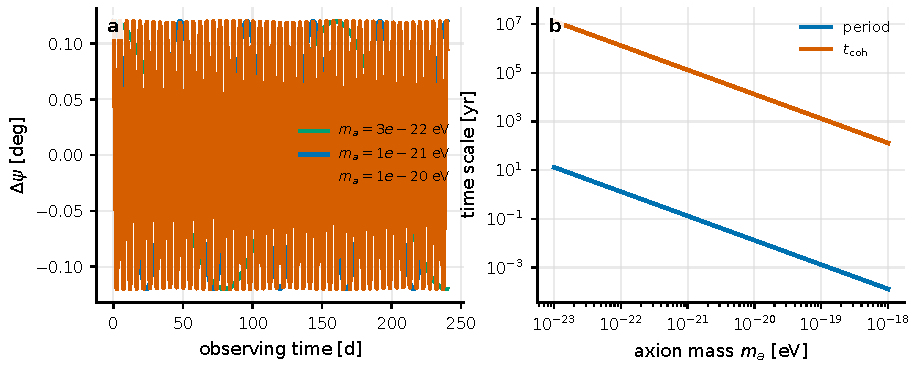
\includegraphics[width=0.94\linewidth]{figures/generated/chapter_15/ch15_axion_polarization_oscillation.pdf}
\caption{Ultralight dark matter turns polarization rotation into a time series. The left panel plots \(\Delta\psi(t)\) for three axion masses: the larger the mass, the faster the oscillation. The right panel converts the mass \(m_a\) into the period \(T_a\) and the coherence time \(t_{\rm coh}\sim T_a/v^2\) (taking \(v=10^{-3}c\)): the lighter the axion, the more slowly it swings, yet the longer it can keep the same phase.}
\label{fig:e22-oscillation}
\end{figure}


\section{How to measure such a small rotation: polarization-resolved intensity and coherence measurements}
\label{sec:e22-measure}

The target signal is often as small as \(10^{-3}\) radians or even smaller. This section makes clear: on what basis, and with what data structure, we catch it, and why ``catching a non-zero angle'' is often first a \emph{systematic-error} problem rather than a discovery.

\paragraph{The essence of polarization measurement: counting photons in a polarization basis}

Back to the foundation laid in Chapter~\ref{chap:e18}: the essence of polarization measurement is to split a beam of light into two (or several) orthogonal polarization channels and \emph{count photons separately}. Keeping accounts with the Stokes parameters (Stokes parameters) \(I,Q,U,V\), the linear-polarization information is all in \(Q\) and \(U\). The action of a polarization rotation \(\beta\) on \(Q,U\) is extremely clean: it multiplies the complex combination \(Q\pm iU\) by a phase factor,

\begin{equation}
  Q\pm iU \;\longrightarrow\; e^{\pm 2i\beta}\,(Q\pm iU).
  \label{eq:e22-qu-rotation}
\end{equation}
\begin{formulaexplain}
\(Q,U\): the linear-polarization Stokes parameters; \(\beta\): the overall polarization rotation angle. The \(2\beta\) (not \(\beta\)) in the exponent comes from the ``spin-2'' nature of linear polarization: polarization is an undirected double arrow, restored by a \(180^\circ\) rotation, so mathematically it appears as \(2\beta\).
\end{formulaexplain}

That \(2\) is crucial: it means a very small angular error is enough to let modes that should be clean contaminate each other. In spherical-harmonic (\(E/B\) mode) space, \eqref{eq:e22-qu-rotation} leaks \(E\) mode into \(B\) mode. If the source's own parity-odd spectrum is negligible, the parity-odd spectrum appearing after rotation is approximately

\begin{equation}
  C_\ell^{EB,\rm obs}=\tfrac12\sin(4\beta)\,(C_\ell^{EE}-C_\ell^{BB}),
  \qquad
  C_\ell^{TB,\rm obs}=\sin(2\beta)\,C_\ell^{TE}.
  \label{eq:e22-eb-tb}
\end{equation}
\begin{formulaexplain}
\(C_\ell^{EB},C_\ell^{TB}\): the parity-odd power spectra that emerge after rotation; \(\beta\): the rotation angle. If the source's intrinsic \(EB/TB\) is very small, a non-zero \(EB/TB\) becomes a probe of the rotation angle, but an error in the detector's angle calibration produces an almost identical shape.
\end{formulaexplain}

\paragraph{Cosmic birefringence: why it is first an angle-calibration problem}

The cosmic microwave background (CMB) is a tempting target for finding a ``global polarization rotation'': the last-scattering surface is extremely far, the sky area extremely large, and the statistics can be pushed very small. But it also forces a simple problem into the sharpest systematic-error problem. The universe itself rotating the polarization by \(\beta\) (cosmic birefringence, cosmic birefringence), and the detector's overall angle calibration being off by \(\alpha\), look almost identical in the CMB spectra: both produce the same-shaped \(EB\) through \eqref{eq:e22-eb-tb}. Plug in a number to feel the strength: at \(\beta=0.35^\circ\), \(\tfrac12\sin(4\beta)\simeq0.012\), that is, the \(EB\) leakage is only of order one percent of \(EE\!-\!BB\), the signal is already weak, and it is entangled with the calibration error. The Planck 2018 reanalysis pried the two partly apart with a clever trick: the CMB rotation \(\beta\) acts only on light from the last-scattering surface, while the Galactic-foreground polarization is right in front of us and is \emph{not} twisted by the cosmic rotation, and the two have different dependences on frequency and multipole, so one can fit \(\beta\) and the calibration angle \(\alpha\) simultaneously, giving \(\beta=0.35\pm0.14^\circ\) (\(68\%\) confidence). Subsequent WMAP+Planck and Planck PR4 analyses have repeatedly stressed that dust's own \(EB\), bandpass mismatch, \(I\to P\) leakage, cross-polarization response, and the choice of sky mask remain the main systematic errors weighing on this result \citep{2020PhRvL.125v1301M,2022NatRP...4..452K,2022PhRvD.106f3503E,2022PhRvL.128i1302D}. The original theoretical basis of cosmic birefringence can be traced to the discussion of pseudoscalar-field-induced optical rotation by Carroll, Field, Jackiw, and others \citep{1990PhRvD..41.1231C,1999PhRvL..83.1506L}.

\begin{figure}[tbp]
\centering
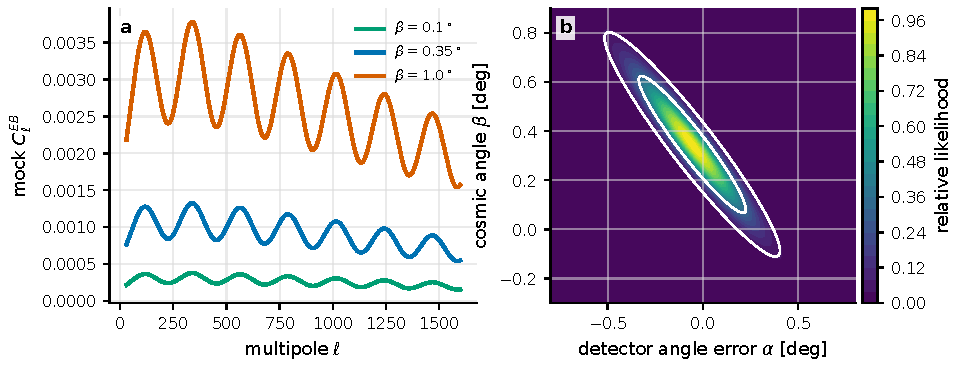
\includegraphics[width=0.94\linewidth]{figures/generated/chapter_15/ch15_cosmic_birefringence.pdf}
\caption{Cosmic birefringence simultaneously moves \(E/B\) mixing and the instrument angle calibration. The left panel uses toy \(EE\), \(BB\) spectra to demonstrate how the rotation angle \(\beta\) generates \(EB\) out of nothing. The right panel plots the degeneracy of the calibration angle \(\alpha\) and the cosmic rotation \(\beta\): looking only at the CMB, the two are nearly equivalent; only by relying on the frequency dependence of the foreground can the degeneracy be broken.}
\label{fig:e22-birefringence}
\end{figure}

\paragraph{Keep the measurement as an event table: do not average too early}

\Needspace{10\baselineskip}
More generally, the most robust approach is not to hurry to average the data into ``a map of a fixed polarization angle,'' but to keep it as a \emph{polarization event table} (following the event-table paradigm of Chapter~\ref{chap:e13}). Each photon event carries a time, frequency, direction, polarization channel, and weight:

\begin{equation}
  e_q=(t_q,\ \nu_q,\ \hat{\bm n}_q,\ p_q,\ w_q).
  \label{eq:e22-event}
\end{equation}
\begin{formulaexplain}
\(e_q\): the \(q\)-th polarization event; \(t_q,\nu_q,\hat{\bm n}_q\): the arrival time, frequency, celestial direction; \(p_q\): which polarization channel it falls into; \(w_q\): the quality weight. Keeping it as an event table lets one search for a ``common rotation'' in the time and frequency dimensions simultaneously, without first averaging away the phase information.
\end{formulaexplain}

If a small common oscillation \(\delta\psi\) is hidden in the polarization angle, the probability of falling into a given polarization channel is written as

\begin{equation}
  P\!\left(p_q\,\middle|\,t_q,\nu_q,\hat{\bm n}_q\right)
  = P_0\!\left[\,p_q\,\middle|\,\psi_{\rm src}
     +\psi_{\rm prop}(\nu_q,\hat{\bm n}_q)+\delta\psi(t_q,\hat{\bm n}_q)\,\right].
  \label{eq:e22-likelihood}
\end{equation}
\begin{formulaexplain}
\(\psi_{\rm src}\): the source's intrinsic polarization angle; \(\psi_{\rm prop}\): the propagation and instrument terms (including Faraday, dust, and the instrument Mueller matrix); \(\delta\psi\): the new-physics rotation to be tested. This likelihood splits the ``anomalous angle'' into several classes of \emph{mutually refutable} sources, put into the same fit together.
\end{formulaexplain}

The price is also frighteningly plain: if the off-diagonal terms of the instrument's Mueller matrix are calibrated only to \(10^{-3}\), while the rotation you seek is also \(10^{-3}\) radians, then the systematic error is already \emph{of the same order} as the signal: at which point a beautiful non-zero angle is most likely the instrument talking, not the universe. The optical polarization of isolated neutron stars, the X-ray polarization of magnetars, and the candidate signal of strong-field QED vacuum birefringence must all first have the source's geometry and propagation effects modeled clean before a polarization anomaly can possibly be interpreted as new physics \citep{2017MNRAS.465..492M}.


\section{Strong-field environments: compact objects as axion laboratories}
\label{sec:e22-strongfield}

The rotation channel relies on the axion field itself; the \emph{conversion} channel requires a strong magnetic field to turn the axion and photon directly into each other. Where are the strongest magnetic fields? Precisely the compact objects (neutron stars, magnetars) of Chapter~\ref{chap:e18} and the black holes of Chapter~\ref{chap:e19}. This section moves the polarization quantum channel into the strong-field environments of neutron stars, magnetars, and black holes, both computing the conversion probability and connecting to the boson cloud of superradiance.

\paragraph{Axion--photon conversion in a magnetic field}

In a transverse magnetic field \(B_\perp\), the axion mixes only with the photon polarization state parallel to \(B_\perp\). With weak mixing, a uniform magnetic field, and negligible absorption, the conversion probability is

\begin{equation}
  P_{a\to\gamma}\simeq\left(\frac{g_{a\gamma}B_\perp L}{2}\right)^2
  \mathrm{sinc}^2\!\left(\frac{qL}{2}\right),
  \qquad
  q\simeq\frac{|m_a^2-m_\gamma^2|}{2E}.
  \label{eq:e22-conversion}
\end{equation}
\begin{formulaexplain}
\(P_{a\to\gamma}\): the probability of an axion turning into a photon; \(B_\perp\): the transverse magnetic field; \(L\): the coherent path length; \(E\): the energy; \(m_\gamma\): the effective mass of the photon in the plasma; \(q\): the momentum mismatch of the axion and photon. The square out front gives the strength, and the \(\mathrm{sinc}^2\) factor governs coherence: once the phase mismatches, the accumulation is cut off.
\end{formulaexplain}

Please look at it side by side with the rotation formula \eqref{eq:e22-rotation}, and the contrast of the two kinds of ``distance dependence'' is clear at a glance. When \(qL\ll1\) (coherent), \(\mathrm{sinc}^2\to1\), and the probability grows as \(L^2\): \textbf{conversion accumulates along the way, the longer the travel the stronger}, which is exactly the opposite of ``rotation cares only about the two endpoints.'' But once \(qL\gtrsim\pi\), the conversion amplitudes of different path segments begin to cancel out of phase, \(\mathrm{sinc}^2\) decays rapidly, and no amount of extra length helps. This is the physics of the coherence length. Ground experiments use this formula to the hilt: CAST uses a decommissioned LHC dipole magnet (\(9\,\mathrm T\), \(9.26\,\mathrm m\)) to stare at the Sun, seeking X-rays converted from solar axions, and its 2013--2015 vacuum-pipe data gives \(g_{a\gamma}<0.66\times10^{-10}\,\mathrm{GeV^{-1}}\) (\(95\%\) confidence), applicable to the coherent low-mass region \(m_a\lesssim0.02\,\mathrm{eV}\) \citep{2017NatPh..13..584C}.

\begin{figure}[tbp]
\centering
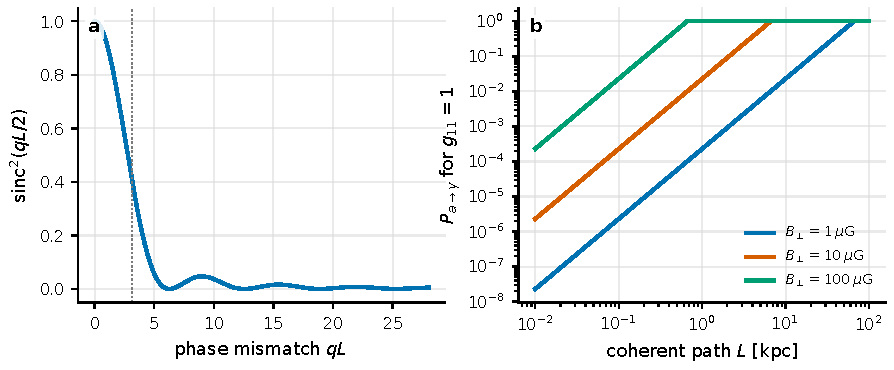
\includegraphics[width=0.94\linewidth]{figures/generated/chapter_15/ch15_axion_conversion.pdf}
\caption{Axion--photon conversion is determined jointly by intensity and phase. The left panel is the coherence factor \(\mathrm{sinc}^2(qL/2)\): as \(qL\) approaches \(\pi\), the conversion amplitudes of different parts of the path begin to cancel. The right panel gives the order of magnitude of the interstellar-scale coherence limit (taking \(g_{a\gamma}=10^{-11}\,\mathrm{GeV^{-1}}\)): in a \(\mu\mathrm G\) field over a kpc path, the single-segment conversion probability is usually far less than 1.}
\label{fig:e22-conversion}
\end{figure}

\paragraph{Magnetars and FRBs: extreme-magnetization polarization laboratories}

Neutron stars and magnetars push all of this to the limit: in Chapter~\ref{chap:e18} we already saw that the magnetic field at a magnetar surface approaches the critical field, and even the vacuum becomes a birefringent medium. This environment is a natural amplifier for axion conversion, but it also means that the intrinsic polarization structure and the propagation foreground are both extremely strong. Fast radio bursts (FRBs) give another class of extreme sample: FRB~121102 lies in a host galaxy at \(z=0.193\), and its \(4\text{--}8\,\mathrm{GHz}\) bursts show nearly \(100\%\) linear polarization, yet carry an absurdly high, time-varying Faraday rotation measure \(\mathrm{RM}_{\rm src}=1.46\times10^5\) and \(1.33\times10^5\,\mathrm{rad\,m^{-2}}\), with individual sub-structures as narrow as \(\lesssim30\,\mu\mathrm s\). If the host contributes \(\mathrm{DM_{host}}\sim70\text{--}270\,\mathrm{pc\,cm^{-3}}\), the inferred lower limit of the line-of-sight magnetic field already reaches order milligauss (mG), several hundred times the \(\sim5\,\mu\mathrm G\) of the ordinary Galactic interstellar medium \citep{2018Natur.553..182M}. This class of source is both a laboratory for extreme-magnetization plasma and the most cunning of impostors: a seemingly ``achromatic'' polarization variation must still first rule out depolarization caused by finite channel width, drift of \(\mathrm{RM}\) with time, and the selection effect of a plasma lens, before it is the axion's turn.

\begin{figure}[tbp]
\centering
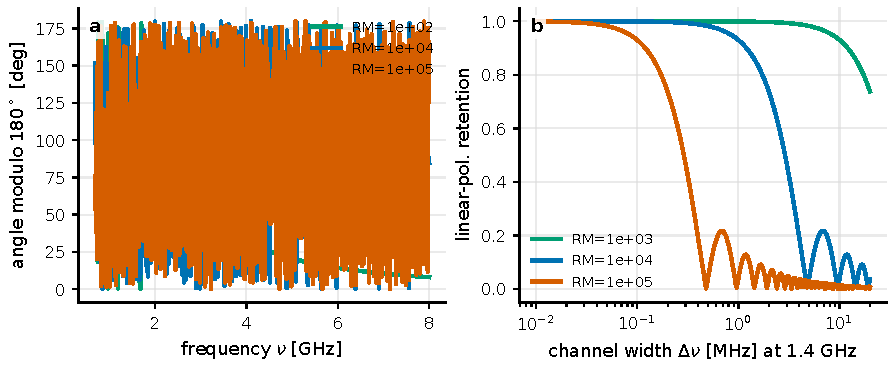
\includegraphics[width=0.94\linewidth]{figures/generated/chapter_15/ch15_frb_faraday_foreground.pdf}
\caption{The polarization foreground of an FRB can easily drown a weak rotation. The left panel plots the \(180^\circ\) wrapping of the polarization angle with frequency under different \(\mathrm{RM}\): \(\mathrm{RM}=10^5\,\mathrm{rad\,m^{-2}}\) varies extremely fast in the GHz band. The right panel is the linear-polarization retention fraction caused by finite channel width near \(1.4\,\mathrm{GHz}\): to measure such a high \(\mathrm{RM}\), one must use extremely narrow channels.}
\label{fig:e22-frb}
\end{figure}

\paragraph{Black hole superradiance: seeding a light boson field beside a spinning black hole}

A black hole ties a light boson field and the polarization picture into one. A boson wave orbiting a spinning (Kerr) black hole, provided its frequency is low enough to satisfy

\begin{equation}
  \omega<m\,\Omega_H,
  \label{eq:e22-superradiance}
\end{equation}
\begin{formulaexplain}
\(\omega\): the boson mode frequency; \(m\): the azimuthal quantum number (integer); \(\Omega_H\): the angular velocity of the Kerr black hole horizon. When this inequality is satisfied, the wave \emph{extracts} energy from the black hole's spin, grows exponentially, and piles up into a boson cloud orbiting the black hole.
\end{formulaexplain}

can extract energy from the black hole's spin, be amplified exponentially, and grow into a ``superradiant boson cloud'' (superradiant boson cloud). Whether the cloud can grow effectively depends on whether the axion Compton wavelength matches the black hole scale. Define a dimensionless ``gravitational fine-structure constant''

\begin{equation}
  \alpha_G=\frac{G M_\bullet m_a}{\hbar c},
  \label{eq:e22-alphaG}
\end{equation}
\begin{formulaexplain}
\(\alpha_G\): the ratio of the black hole gravitational radius to the axion Compton wavelength; \(M_\bullet\): the black hole mass. When \(\alpha_G\sim0.1\text{--}1\), the boson wave ``fits'' near the black hole, and superradiant growth is fastest.
\end{formulaexplain}

When \(\alpha_G\sim0.1\text{--}1\), the boson Compton wavelength matches the black hole scale, and the cloud grows most fiercely. Inverting \eqref{eq:e22-alphaG} maps the black hole mass to the axion mass it is most sensitive to:

\begin{equation}
  m_a\simeq 1.34\times10^{-10}\,\mathrm{eV}\;\alpha_G
  \left(\frac{M_\odot}{M_\bullet}\right).
  \label{eq:e22-bh-mass}
\end{equation}
\begin{formulaexplain}
Converting the black hole mass \(M_\bullet\) into the most-sensitive axion mass \(m_a\): the heavier the black hole, the lower the corresponding axion-mass window. So black holes of different mass probe different segments of the ultralight-mass spectrum.
\end{formulaexplain}

Take two real black holes. The Galactic-center Sgr~A\(^*\) (\(4.3\times10^6\,M_\odot\)) at \(\alpha_G=0.4\) corresponds to \(m_a\simeq1.2\times10^{-17}\,\mathrm{eV}\); M87\(^*\) (\(6.5\times10^9\,M_\odot\)) corresponds to \(8\times10^{-21}\,\mathrm{eV}\): the two black holes probe completely different mass segments. Here the polarization channel returns again: in EHT polarization imaging, an axion cloud makes the polarization angle on the ring swing together with the axion period, with Sgr~A\(^*\)'s period about \(100\text{--}1000\,\mathrm s\) and M87\(^*\)'s reaching several days. Whether this swing can be seen depends on the spatial resolution: if the different azimuths on the ring cannot be resolved, the swing is ``averaged'' out \citep{2015LNP...906.....B,2015CQGra..32m4001B,2017PhRvD..96c5019B,2020PhRvL.124f1102C,2022NatAs...6..592C}.

\begin{figure}[tbp]
\centering
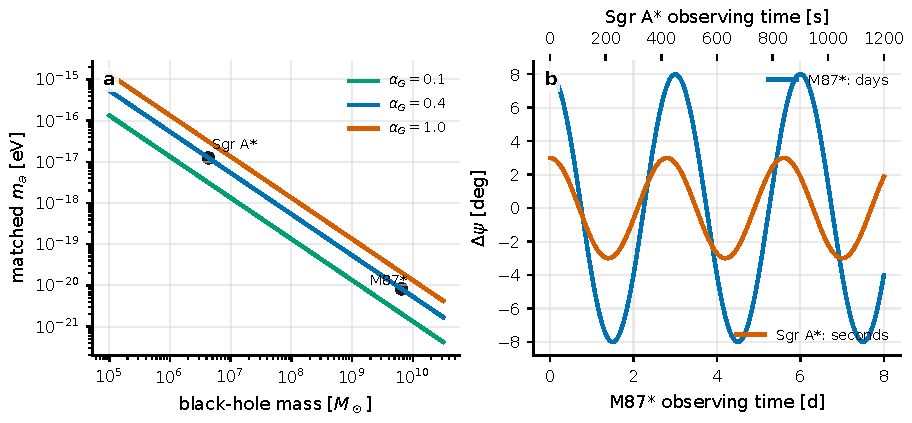
\includegraphics[width=0.94\linewidth]{figures/generated/chapter_15/ch15_black_hole_axion_cloud.pdf}
\caption{The black hole mass frames the mass window of the superradiant axion. The left panel uses \(\alpha_G=GM_\bullet m_a/\hbar c\) to mark the \(m_a\) corresponding to different black hole masses: Sgr~A\(^*\) and M87\(^*\) fall in different ultralight-mass segments. The right panel gives two typical timescales of the EHT polarization-angle oscillation: M87\(^*\) can be sampled on the day scale, while Sgr~A\(^*\) requires second-to-minute-scale polarization imaging.}
\label{fig:e22-bh}
\end{figure}


\section{Writing the anomaly as a refutable test}
\label{sec:e22-falsifiable}

By this point, all candidate signals share one iron law: \textbf{the anomaly itself is not the conclusion; the ``refutable structure'' of the anomaly is the conclusion}. This section gathers the tricks scattered above into a unified ledger.

\paragraph{One ledger: spread out and align the four classes of source}

The observables of a new-physics search are often more than one: polarization angle, arrival time, image position, magnification, possibly from different instruments, each carrying its own statistical and systematic error. Combining them into one data vector \(\bm d\), the model splits into four major blocks:

\begin{equation}
  \bm m(\bm\theta)=\bm m_{\rm src}+\bm m_{\rm prop}+\bm m_{\rm inst}+\bm m_{\rm new}(\bm\theta),
  \label{eq:e22-model-vector}
\end{equation}
\begin{formulaexplain}
\(\bm m\): the model prediction vector; the four terms are the source, propagation, instrument, and new physics. \(\bm\theta\): the new-physics parameters (\(g_{a\gamma}\), \(m_a\), \(\beta\), the subhalo mass function, etc.). This decomposition forces us to compare the anomaly with ordinary astrophysics, propagation foregrounds, and calibration errors in \emph{the same ledger}.
\end{formulaexplain}

In the Gaussian approximation, the objective function of the fit is

\begin{equation}
  -2\ln\mathcal L=\big[\bm d-\bm m(\bm\theta)\big]^{\mathsf T}
  \big(C_{\rm stat}+C_{\rm sys}\big)^{-1}
  \big[\bm d-\bm m(\bm\theta)\big]
  +\ln\det\big(C_{\rm stat}+C_{\rm sys}\big).
  \label{eq:e22-likelihood-gauss}
\end{equation}
\begin{formulaexplain}
\(\mathcal L\): the Gaussian likelihood; \(C_{\rm stat}\): the statistical covariance (photon noise, arrival-time error, image noise); \(C_{\rm sys}\): the systematic-error covariance (Mueller matrix, absolute polarization angle, Faraday foreground, dust \(EB\), lens macromodel, \ldots). The residual must be weighted by \emph{both} classes of error together; omit \(C_{\rm sys}\), and an isolated anomaly will be wrongly amplified.
\end{formulaexplain}

This expression makes mathematical the sentence this chapter keeps repeating: as long as \(C_{\rm sys}\) is not in the likelihood, any single anomalous point will be over-interpreted.

\paragraph{Five crowbars: making different signals betray one another}

Fortunately these signals have clear ways of distinguishing one another, and each corresponds to physics discussed earlier:

\begin{itemize}
\item \textbf{Wavelength dependence.} Faraday rotation goes as \(\lambda^2\) (Chapter~\ref{chap:e21}), axion rotation is approximately achromatic (\eqref{eq:e22-rotation}): measuring at several frequencies pries them apart.
\item \textbf{Temporal behavior.} Static cosmic birefringence gives an unchanging global angle (\eqref{eq:e22-eb-tb}), ultralight dark matter gives a breathing sinusoid (\eqref{eq:e22-osc-signal}): measuring over tens of days to years pries them apart.
\item \textbf{Black hole scaling.} The polarization oscillation of the superradiant cloud should be linked to the black hole mass, spin, azimuth on the ring, and observing time (\eqref{eq:e22-bh-mass}); an ordinary accretion flow does not so ``obey the black hole.''
\item \textbf{Path dependence.} Conversion accumulates along the way as \(L^2\) (\eqref{eq:e22-conversion}), while rotation cares only about the two endpoints: the distance responses of the two are exactly opposite.
\item \textbf{Cross-checks.} Sample statistics, blank fields or control sources, frequency inversion, temporal coherence, instrument recalibration: if any one of these fails, the ``discovery'' should be downgraded.
\end{itemize}

\paragraph{A parallel channel: how dark matter turns mass into an angular offset}

The polarization channel seeks ``the quantum effect of a field on photons''; there is also a parallel channel, seeking ``the effect of the dark-matter mass distribution on the light path'': gravitational lensing. It is likewise ``achromatic,'' likewise manifested not as ``seeing a clump of dark matter'' but as an image position, magnification, or arrival time deviating from the ordinary model. The existence of dark matter itself has multiple supports: galaxy-cluster collisions (such as the separation of the weak-lensing mass peak from the X-ray gas in the Bullet Cluster, indicating that the main mass is approximately collisionless), weak lensing, and dynamics \citep{2006ApJ...648L.109C,1993ApJ...404..441K}; and cold-dark-matter simulations predict that the Galactic halo is full of subhalos far below the visible satellite galaxies, becoming an important candidate explanation for strong-lensing anomalies \citep{1994ApJ...427L...1F,1999ApJ...524L..19M,2008Natur.454..735D}. The order of magnitude of subhalo lensing is given by the Einstein angle,

\begin{equation}
  \theta_E=\left(\frac{4GM}{c^2}\frac{D_{ls}}{D_lD_s}\right)^{1/2},
  \qquad
  \delta\theta\simeq\frac{\theta_E^2}{b},
  \label{eq:e22-lensing}
\end{equation}
\begin{formulaexplain}
\(\theta_E\): the subhalo Einstein angle, \(\propto M^{1/2}\); \(M\): the lens mass; \(D\): the combination of observer--lens--source distances; \(\delta\theta\): the astrometric offset of the image; \(b\): the angular distance of the image from the subhalo (\(b\gg\theta_E\)). The larger the mass and the closer to the image, the more marked the position perturbation; far away it decays as \(1/b\).
\end{formulaexplain}

The numbers set the resolution requirement very hard: in a galaxy strong lens with \(D_l\simeq1\,\mathrm{Gpc}\), \(D_s\simeq2\,\mathrm{Gpc}\), the \(\theta_E\) of a \(10^8\,M_\odot\) subhalo is a few tens of milliarcseconds (mas), and a \(10^6\,M_\odot\) one is only a few mas; while a \(10^6\,M_\odot\) subhalo at \(b=10\,\mathrm{mas}\) gives an astrometric offset of only order \(\mu\mathrm{as}\). The flux-ratio anomalies of strong lensing are sensitive to magnification perturbations: Mao and Schneider pointed out that low-mass substructure can explain the anomalies of some quadruple-image systems, Dalal and Kochanek used 7 radio lenses to measure a median substructure mass fraction \(f_{\rm sat}\simeq0.02\) (\(90\%\) range about \(0.006\text{--}0.07\)), and Vegetti, Hezaveh, and others used gravitational imaging and ALMA to push the detection of a single dark substructure to spatially resolved modeling \citep{1998MNRAS.295..587M,2002ApJ...572...25D,2010MNRAS.408.1969V,2016ApJ...823...37H}; Gaia and future astrometric surveys turn a subhalo transiting a background source into a time-domain signal, with the main limits coming from the scanning law, source density, and proper-motion covariance \citep{2024MNRAS.531..632M,2016PhRvD..94h3504C}. The ledger of this channel is entirely consistent with that of the polarization channel (\eqref{eq:e22-model-vector}): a dark subhalo should \emph{simultaneously} perturb the image position, magnification, and time delay, whereas stellar-surface structure varies mainly with source rotation, wavelength, and baseline direction. Put these distinctions into the same likelihood, and only then can an anomaly be upgraded to a discovery.

\begin{figure}[tbp]
\centering
\includegraphics[width=0.94\linewidth]{figures/generated/chapter_15/ch15_dark_matter_lensing.pdf}
\caption{The lensing signal of a dark-matter subhalo is limited by angular scale. The left panel gives the variation of the subhalo Einstein angle with mass for a typical Gpc geometry. The right panel converts \(\delta\theta\simeq\theta_E^2/b\) into an astrometric offset: a low-mass subhalo requires mas-level proximity and \(\mu\mathrm{as}\)-level systematic control to possibly be seen.}
\label{fig:e22-lensing}
\end{figure}

\paragraph{A time-domain corroboration: pulsar arrays}

The same ``common time term'' logic can also be used on pulsars. Pulsars have stable phases and repeating pulses, naturally suited to a time-domain array (pulsar timing array, PTA). The oscillation of the gravitational potential of ultralight scalar dark matter leaves a narrowband signal in the timing residuals: writing it as \(\Psi_c\cos(2m_at+\varphi)\), the simplified residual is

\begin{equation}
  R_\alpha(t)\simeq\frac{\Psi_c}{2\pi f}
  \Big[\sin(2\pi ft+\varphi_E)-\sin\!\big(2\pi f(t-D_\alpha/c)+\varphi_\alpha\big)\Big],
  \label{eq:e22-pta}
\end{equation}
\begin{formulaexplain}
\(R_\alpha\): the timing residual of the \(\alpha\)-th pulsar; \(\Psi_c\): the potential-oscillation amplitude; \(f\simeq m_a/\pi\): the narrowband frequency; \(D_\alpha\): the pulsar distance. The first term is the ``Earth term'' shared by all pulsars, and the second is each star's own ``pulsar term.''
\end{formulaexplain}

\(m_a\sim10^{-23}\,\mathrm{eV}\) corresponds to \(f\sim10^{-8}\,\mathrm{Hz}\), falling right in the PTA window of \(10^{-9}\text{--}10^{-7}\,\mathrm{Hz}\). Porayko and Postnov analyzed old NANOGrav data and gave an upper limit \(\Psi_c<1.14\times10^{-15}\) (\(95\%\) confidence) \citep{2014PhRvD..90f2008P}. The inter-pulsar correlation of this scalar template hardly depends on the angle between two stars, and is therefore different from the famous Hellings--Downs angular-correlation curve of a stochastic gravitational-wave background: this is itself another crowbar. If a ``pulsar polarization array'' is done in the future, one must likewise separate out the common Earth term, the intrinsic magnetospheric polarization, the interstellar Faraday rotation, pulse-profile variations, and receiver polarization leakage one by one.

\begin{figure}[tbp]
\centering
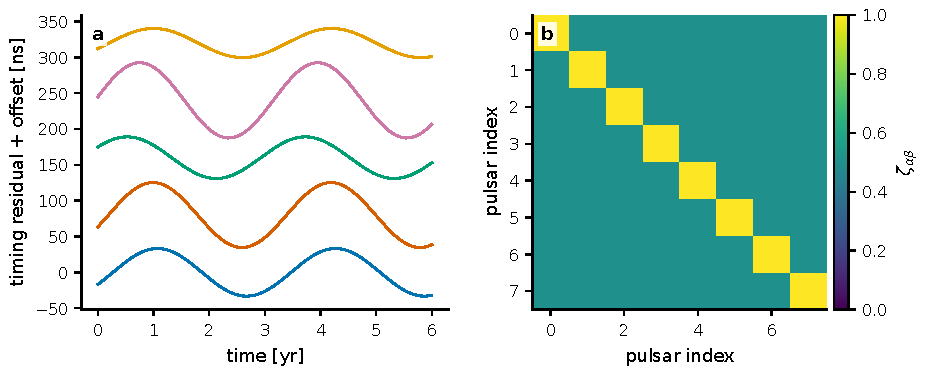
\includegraphics[width=0.94\linewidth]{figures/generated/chapter_15/ch15_pulsar_array_correlation.pdf}
\caption{The common narrowband signal in a pulsar array. The left panel is a common Earth term superimposed on each star's own pulsar term (the curves are artificially offset for viewing). The right panel gives the simplified correlation matrix of the scalar-potential-oscillation model \(\zeta_{\alpha\beta}=(1+\delta_{\alpha\beta})/2\), which differs from the angular correlation of a stochastic tensor gravitational-wave background.}
\label{fig:e22-pta}
\end{figure}


\section{Chapter Summary}
\label{sec:e22-summary}

\begin{itemize}
\item \textbf{One coupling, two observables.} The minimal \(a\,\bm E\cdot\bm B\) coupling (\eqref{eq:e22-lagrangian}) opens two quantum channels simultaneously: the axion background \emph{twists} the plane of linear polarization, and in a strong magnetic field the axion and photon \emph{convert} into each other. Both measure polarization, yet the physics is complementary.
\item \textbf{The rotation angle cares only about the two endpoints, and is achromatic.} The phase difference is the integral of a total differential along the path, leaving only the endpoint difference (\eqref{eq:e22-phase-diff}), and the rotation angle is half of it (\eqref{eq:e22-rotation}), and it \emph{contains no wavelength}: this is the first crowbar that separates it from Faraday rotation (\(\propto\lambda^2\)).
\item \textbf{Dark matter makes polarization breathe.} If the axion is ultralight dark matter, the field oscillates with time (\eqref{eq:e22-dm-field}), and the rotation angle becomes a quasi-monochromatic sinusoid (\eqref{eq:e22-osc-signal}); the period is tens of days and the coherence time can reach \(10^5\) years (\eqref{eq:e22-timescales}): the search must look for a common swing over a long time baseline, not measure only once.
\item \textbf{The essence of measurement is counting photons in a polarization basis.} The \(2\beta\) of Stokes rotation (\eqref{eq:e22-qu-rotation}) leaks \(E\) into \(B\) (\eqref{eq:e22-eb-tb}); CMB birefringence is first a degeneracy problem between \(\beta\) and the calibration angle \(\alpha\), and the result \(\beta=0.35\pm0.14^\circ\) relies entirely on the foreground frequency dependence to break the degeneracy. Keeping the data as an event table (\eqref{eq:e22-event}, \eqref{eq:e22-likelihood}) avoids averaging away the signal too early.
\item \textbf{Conversion accumulates along the way, and compact objects are amplifiers.} \(P_{a\to\gamma}\propto(g_{a\gamma}B_\perp L)^2\,\mathrm{sinc}^2(qL/2)\) (\eqref{eq:e22-conversion}) grows as \(L^2\) in the coherent region; the extreme magnetization of magnetars and FRBs and the black hole superradiant boson cloud (\eqref{eq:e22-superradiance}--\eqref{eq:e22-bh-mass}) move the polarization channel into strong fields, at the price of an equally fierce intrinsic structure and foreground.
\item \textbf{An anomaly must be written as a refutable ledger.} Split the source, propagation, instrument, and new physics apart (\eqref{eq:e22-model-vector}), and weight with \(C_{\rm stat}+C_{\rm sys}\) together (\eqref{eq:e22-likelihood-gauss}); rely on the five crowbars of wavelength, time, black hole scaling, path dependence, and cross-checks to make the signals betray one another. Lensing (\eqref{eq:e22-lensing}) and PTA (\eqref{eq:e22-pta}) are parallel channels of the same logic.
\end{itemize}

\noindent\textbf{Questions to Ponder.}
(1) Why does the field value ``in the middle of the path'' not appear at all in the axion rotation formula \eqref{eq:e22-rotation}, while the conversion formula \eqref{eq:e22-conversion} is extremely sensitive to the path length \(L\)? How can this difference in the two kinds of ``distance dependence'' help you separate them in real data?
(2) If a telescope's polarization-angle calibration error is \(0.5^\circ\) and the cosmic birefringence you seek is \(0.35^\circ\), do you have any way, using \emph{only} this one instrument, to separate the two? Why can ``using the frequency dependence of the foreground'' come to the rescue?
(3) Sgr~A\(^*\) and M87\(^*\) probe completely different axion-mass segments (\eqref{eq:e22-bh-mass}). Suppose one day you see the polarization angle on M87\(^*\)'s ring oscillating with a period of several days; would you first suspect it is an axion cloud, or first suspect the accretion flow itself? Which cross-checks would you need before you dare to upgrade it to a ``discovery''?
